\documentclass[a4paper,man,natbib,floatsintext,12pt]{apa7}

\usepackage[english]{babel} %character and hyphenation rules specific to the language you choose
%\usepackage[utf8x]{inputenc}
\usepackage{graphicx}
\usepackage{color}
\usepackage{tikz}
\usepackage{amsmath}
\usepackage{blindtext}
\usepackage{tabularx} %great for APA-style Tables
\usepackage{siunitx} % Required for good table alignmen
\sisetup{
  round-mode          = places, % Rounds numbers
  round-precision     = 2, % to 2 places
}
\usepackage{multirow}
\usepackage{booktabs}
\usepackage{wrapfig}
\usetikzlibrary{shapes,decorations,arrows,calc,arrows.meta,fit,positioning}
\tikzset{
    -Latex,auto,node distance =1 cm and 1 cm,semithick,
    latent/.style ={ellipse, draw, minimum width = 0.7 cm},
    observed/.style ={rectangle, draw},
    bidirected/.style={Latex-Latex,dashed},
    el/.style = {inner sep=2pt, align=left, sloped}
}
\newcommand{\sigFtest}[4]{\textit{F}(#1,#2) = #3, \textit{p}$<$#4}
\newcommand{\nonsigFtest}[3]{\textit{F}(#1,#2) = #3, \textit{p}$>$.05}


\title{Examining Emotional and Psychological Outcomes of a Modified Tuning in to Teens\textsuperscript{®} Program}
\shorttitle{Emotional and Psychological Outcomes of TINT}
\author{Natalie Tuinstra}
\affiliation{College of William \& Mary}
\journal{The Best Psychology Journal EVER!}
\abstract{Early adolescence is a key developmental stage during which symptoms of anxiety, depression, and behavioral difficulties often intensify. Emotional competency skills, such as awareness, expression, and coping, play a vital role in mitigating these risks. The present study examined the effects of a modification of the Tuning in to Teens® (TINT) program (Kehoe et al., 2014), traditionally designed for parents, but now adapted for direct involvement of a community sample of middle-school-age adolescents. Participants were 45 youth (Mage= 11.79 years; 57.8\% girls; 75.6\% White) who participated in six weekly, two-hour group sessions focused on teaching emotional competency skills related to anger, sadness, and worry. Adolescents and their caregivers completed emotion skills and psychopathology measures at baseline (T1), post-intervention (T2), and one-month follow-up (T3). Adolescents reported significant improvements in emotion regulation coping and reductions in internalizing and externalizing symptoms. Parents observed gains in emotional awareness, expression, and regulation, along with fewer externalizing behaviors. Emotion-specific patterns emerged: across time, worry was more inhibited than anger and sadness, yet more effectively regulated. In contrast, anger and sadness were more likely to be expressed in dysregulated ways and less likely to demonstrate consistent improvement in regulation. These findings offer preliminary evidence for the short-term benefits of this modified TINT program that appears to support adolescent emotional and psychological well-being.}
\keywords{intervention, emotion regulation, psychopathology}
\authornote{I would like to thank my dog, George, for taking a nap while I worked on this.}
\leftheader{Alternate page header in man mode}

%-------------- END PREAMBLE  -------------------


\begin{document}

\maketitle  %Insert my APA style title page


Adolescence is a developmental period characterized by rapid biological, cognitive, and socio-emotional changes that shape mental health trajectories. During this time, youth face increased vulnerability to the onset of psychological disorders, in part due to heightened emotional reactivity and evolving social-cognitive capacities \citep{jaworska2015adolescent}. Emotional awareness, or the ability to identify, differentiate, and understand one’s emotional experiences, has been shown to be a transdiagnostic predictor of internalizing symptoms such as depression and anxiety \citep{kranzler2016emotional}. Deficits in these competencies may also exacerbate externalizing difficulties by undermining youths’ capacity for effective regulation.

Research highlights the importance of emotion regulation in promoting adaptive development and reducing risk for psychopathology. Foundational work suggests that effective regulation of emotions is associated with positive social and psychological adjustment, while poor regulation predicts maladaptive outcomes \citep{eisenberg2001relations}. Furthermore, studies of emotion processing indicate that attentional mechanisms influence how adolescents encode and respond to emotional information, linking cognitive processes with socio-emotional functioning \citep{brenner2014role}.

Intervention research has increasingly focused on targeting these emotion skills. For example, the Tuning in to Teens (TINT) program aims to improve parents’ emotion coaching, which has been associated with reductions in adolescent internalizing difficulties \citep{kehoe2014tuning}. Building on this framework, the current study evaluates a modified version of TINT adapted for early adolescents, with a focus on strengthening emotion competencies to reduce internalizing and externalizing symptoms.

We advance two primary hypotheses. First, we expect adolescents will demonstrate improvements in emotional competence—specifically emotional awareness, reduced inhibition and dysregulation, and greater use of adaptive coping strategies—following participation in the program. Second, we expect reductions in internalizing and externalizing symptoms across the same period. Together, these hypotheses test whether directly targeting emotion skills can improve psychological functioning in early adolescence.



\section{Method}
\subsection{Participants}
Participants were recruited from the Williamsburg, Virginia community and were required to be fluent in English and enrolled in 5th, 6th, or 7th grade. The final sample consisted of 45 adolescents (Mage= 11.79 years, SD = 11.41 months; n = 26 girls, 57.8\%) in 5th (n = 14, 31.1\%.), 6th (n = 18, 40\%), and 7th (n = 13, 28.9\%) grades. The sample was predominantly White (n = 34, 75.6\%; Other/Multiracial, n = 7, 15.6\%; Asian, n = 3, 6.7\%; Black, n = 1, 2.2\%). 
In addition to adolescent participants, their primary caregivers provided data (Mage= 41.34 years, SD = 9.19 years; 36 mothers, 9 fathers). However, six caregivers did not complete all three time points, resulting in a final caregiver sample of 39 (Mage= 41.08 years, SD = 9.56 years; 32 mothers, 7 fathers). Specifically, one caregiver did not complete T2 questionnaires, while the remaining five did not complete T3. 
\subsection{Measures}
\subsubsection{Emotion Measures}
\textbf{Emotion Expression Scale for Children (EESC).} The EESC  is a 16-item questionnaire that uses a 5-point response scale (1 = not at all true to 5 = extremely true). The questionnaire is comprised of two subscales of eight items each. The Poor Awareness subscale assesses children’s difficulty in identifying emotions (e.g., “I often do not know how I am feeling.”). Higher scores indicate greater difficulty in emotional awareness. The Expressive Reluctance subscale assesses hesitancy in expressing emotions (e.g., “I prefer to keep my emotions to myself.”). Higher scores suggest greater reluctance to express emotions. The EESC has demonstrated high internal consistency in a community sample of early adolescents, and has shown validity through correlations with measures of emotion management. In the present study, reliability for these child-report scales were acceptable across all three time points, with internal consistencies ranging from .77 to .89. 
A parent-report version of the EESC  was also administered to gain parent perspectives on their child’s emotional awareness and expression. Parents completed the same 16-item measure, rating their child’s tendencies using the identical 5-point response scale. The EESC-P has demonstrated strong internal consistency and predictive validity in prior research (Kerns et al., 2014). In the current study, reliability for these parent-report scales was acceptable, with internal consistencies ranging from .69 to .84.


\section{Results}
\subsection{Emotional Awareness and Expressive Reluctance}
\subsubsection{Child-Report} 

The analyses revealed no significant interaction between time × subscales, F(2, 43) = .10, p = .91, ηp² = .01. Results indicated no significant main effect of time, F(2, 43) = 1.62, p = .21, ηp² = .07. However, there was a significant main effect for subscale type, F(1, 44) = 20.08, p < .001, ηp² = .31, indicating differences in levels of poor awareness and expressive reluctance, independent of time. 

To further investigate these effects, a paired-samples t-test was conducted to compare scores on the poor awareness and expressive reluctance subscales. Results indicated that the average scores on the expressive reluctance subscales (M = 22.94, SD = 6.26) were significantly higher than average scores on the poor awareness subscales (M = 19.62, SD = 7.28), t(45) = 4.48, p < .001 (see Figure~\ref{fig:TikZmodel}). See Table~\ref{tab:child_outcomes} for child-report means and standard deviations.

\begin{figure}[H]
\centering
\resizebox{\textwidth}{!}{%
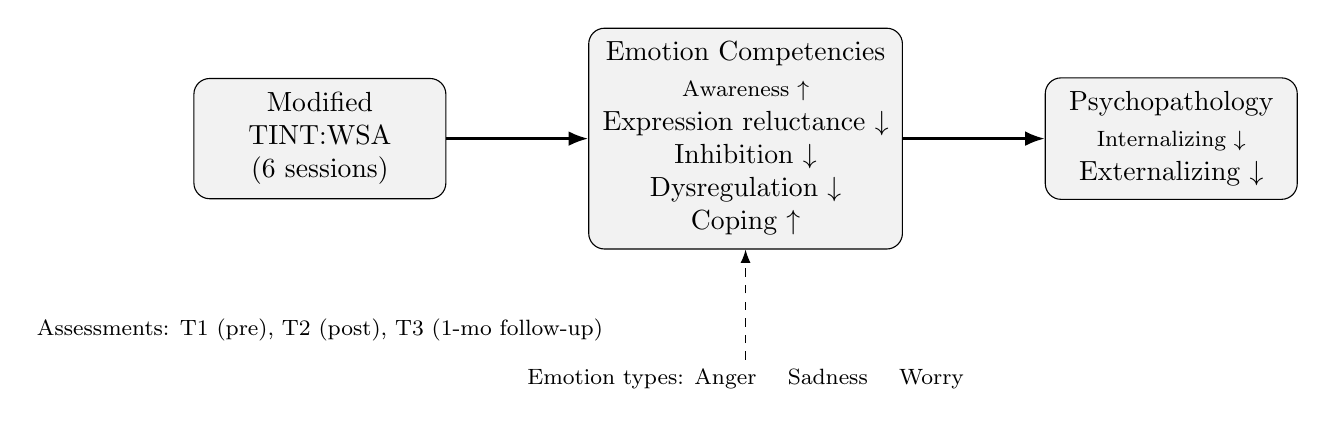
\begin{tikzpicture}[
  node distance=18mm,
  box/.style={draw, rounded corners=2mm, align=center, inner sep=5pt, minimum width=3.2cm},
  >={Latex}
]
% Nodes
\node[box, fill=gray!10] (int) {Modified\\ TINT:WSA\\ (6 sessions)};
\node[box, right=18mm of int, fill=gray!10] (skills) {Emotion Competencies\\[1pt]
\footnotesize Awareness $\uparrow$\\ Expression reluctance $\downarrow$\\ Inhibition $\downarrow$\\ Dysregulation $\downarrow$\\ Coping $\uparrow$};
\node[box, right=18mm of skills, fill=gray!10] (symp) {Psychopathology\\[1pt]
\footnotesize Internalizing $\downarrow$\\ Externalizing $\downarrow$};

% Arrows without labels
\draw[->, line width=0.9pt] (int) -- (skills);
\draw[->, line width=0.9pt] (skills) -- (symp);

% Moderators / emotion types
\node[below=14mm of skills, align=center, font=\footnotesize] (emo)
{Emotion types: Anger \quad Sadness \quad Worry};
\draw[->, dashed] (emo.north) -- (skills.south);

% Notes (timepoints)
\node[below=14mm of int, font=\footnotesize, align=center] (tpts)
{Assessments: T1 (pre), T2 (post), T3 (1-mo follow-up)};
\end{tikzpicture}%
}
\caption{Conceptual model: The modified TINT:WSA aims to enhance adolescents' emotion competencies, which in turn reduce internalizing and externalizing symptoms. }
\label{fig:TikZmodel}
\end{figure}

\begin{table}[H]
\centering
\caption{Means, Standard Deviations, and RM-ANOVAs for the Child-Report Outcomes}
\label{tab:child_outcomes}
\begin{tabular}{lccccccccc}
\toprule
\multirow{2}{*}{Measure} & \multicolumn{2}{c}{T1} & \multicolumn{2}{c}{T2} & \multicolumn{2}{c}{T3} & \multirow{2}{*}{F} & \multirow{2}{*}{p} & \multirow{2}{*}{$\eta_p^2$} \\
 & M & SD & M & SD & M & SD & & & \\
\midrule
\textbf{EESC} & & & & & & & & & \\
\quad PA & 20.27 & 8.00 & 19.31 & 7.62 & 19.29 & 7.72 & 1.01 & .37 & .05 \\
\quad ER & 23.60 & 6.24 & 22.78 & 7.23 & 22.44 & 6.85 & 1.12 & .34 & .06 \\
\textbf{CAMS} & & & & & & & & & \\
\quad Inh. & 1.88 & 0.59 & 1.84 & 0.57 & 1.91 & 0.57 & 0.63 & .51 & .01 \\
\quad Dys. & 1.61 & 0.45 & 1.70 & 0.59 & 1.67 & 0.64 & 0.91 & .40 & .02 \\
\quad Cop. & 2.11 & 0.53 & 2.28 & 0.48 & 2.26 & 0.56 & 3.53 & .04 & .14 \\
\bottomrule
\end{tabular}
\end{table}


\section{Discussion}

\begin{wrapfigure}{l}{0.4\textwidth}     \centering       

\includegraphics[width=0.25\textwidth]{TINT.png}
\caption{\label{fig:TINT} TINT Logo.}
\end{wrapfigure}

The purpose of the present study was to evaluate the outcomes of a modified version of the TINT:WSA program, adapted to teach emotion skills directly to early adolescents rather than solely to parents (see Figure~\ref{fig:TINT} for the program logo). This study extends prior research in several ways. Unlike previous implementations that primarily targeted parents with the expectation that they would transfer learned skills to their children through emotion socialization, this study provided direct instruction to adolescents regarding their emotional awareness, emotional understanding, and emotion regulation strategies. The program also addressed the role of emotions within the context of peer and friendship interactions, a particularly salient domain for early adolescents. 






\bibliography{references.bib}

\end{document}